%
% File naaclhlt2016.tex
%

\documentclass[11pt,letterpaper]{article}
\usepackage{styles/naaclhlt2016}
%\usepackage{styles/naaclhlt2013levi}
\usepackage{times}
\usepackage{latexsym}
\setlength\titlebox{6.5cm}    % Expanding the titlebox

\naaclfinalcopy

\usepackage{rotating}
\usepackage{tikz}
\usetikzlibrary{shapes,arrows}
\usepackage{graphicx}
\usepackage{tikz-dependency}
\usepackage{natbib}
\usepackage{url}
\usepackage{amsmath}
\DeclareMathOperator*{\argmax}{arg\,max}
\DeclareMathOperator*{\argmin}{arg\,min}
\usepackage{tikz-qtree}

\usepackage{multirow}
\usepackage{rotating}
\usepackage{booktabs}

% MD: some versions of latex need this package to be loaded last
\usepackage{gb4e}

\newcommand{\param}[1]{\texttt{#1}}
\newcommand{\md}[1]{\marginpar{\scriptsize MD: #1}}
\newcommand{\lk}[1]{\marginpar{\scriptsize LK: #1}}
% for removing all marginpars ==> good for final submission! %%nice trick!
\renewcommand{\marginpar}[1]{}

%\title{Dependency Vector Comparison for Content Assessment (title?)}
%\title{Bag-of-Dependencies Approaches to Content Assessment (title?)}

% MD: title is too bulky, but may be getting closer?
\title{Shallow Semantic Reasoning from an Incomplete Gold Standard for
  Learner Language}

% Author information can be set in various styles:
% For several authors from the same institution:
\author{Levi King \and Markus Dickinson \\
         Indiana University \\ Bloomington, IN \\ \{\texttt{leviking},\texttt{md7}\} \texttt{@indiana.edu}}
% if the names do not fit well on one line use
%         Author 1 \\ {\bf Author 2} \\ ... \\ {\bf Author n} \\
% For authors from different institutions:
% \author{Author 1 \\ Address line \\  ... \\ Address line
%         \And  ... \And
%         Author n \\ Address line \\ ... \\ Address line}
% To start a seperate ``row'' of authors use \AND, as in
% \author{Author 1 \\ Address line \\  ... \\ Address line
%         \AND
%         Author 2 \\ Address line \\ ... \\ Address line \And
%         Author 3 \\ Address line \\ ... \\ Address line}
% If the title and author information does not fit in the area allocated,
% place \setlength\titlebox{<new height>} right after
% at the top, where <new height> can be something larger than 2.25in
%\author{Author 1\\
%	    XYZ Company\\
%	    111 Anywhere Street\\
%	    Mytown, NY 10000, USA\\
%	    {\tt author1@xyz.org}
%	  \And
%	Author 2\\
%  	ABC University\\
%  	900 Main Street\\
%  	Ourcity, PQ, Canada A1A 1T2\\
%  {\tt author2@abc.ca}}

\date{}

%%%RE: Item 6 and examples: Old way cannot handle the variation where some users use the woman as the object, others use the painting as the object; new method can cover some of this info, but maybe it goes too far? The tension between specificity and abstraction, and strict matching and relaxed matching.
%%%%%Maybe using 'grandparents' (dependency chains) could help... from "painting a portrait of a woman", looking at grandparents could find a relation between 'painting' and 'woman'... would we want to compare grandparents only with grandparents? or with parents? ...

%%%If it comes up, we simply don't have enough data to do machine learning approaches to determine what is relevant in the images or responses
%%%WRT clustering, if we want to do machine learning in the future, our cluster results show that there are different item types, which may need different types of processing... so a machine learning approach would require a lot of *varied* data... maybe multiple classifiers, one per cluster?

%%%Guo Chuen mentioned the possibility of clustering the GS responses within an individual PDT item and trying to match responses to one of these clusters... Something to think about...

%%%Can's comment: look into machine translation evaluation: BLEU scores, METEOR, LEPOR, etc. Would anything from ML be appropriate here? The GS and the NNS would both be treated as translations from the image.... We allow for grammatical variability in ways that MT doesn't allow, also n-gram matching might not be good for us; for us, knowing *number* of similar responses is important (saliency, relevancy, etc.), but in MT, a single matching instance is enough; pictures allow for more interpretation than a source sentence -- this may point us toward paraphrase work instead.


\begin{document}

\maketitle

\begin{abstract}
  We investigate questions of how to reason about learner meaning in
  cases where the set of correct meanings is never entirely complete,
  specifically for the case of picture description tasks (PDTs).  To
  operationalize this, we explore different models of representing and
  scoring non-native speaker (NNS) responses to a picture, including
  bags of dependencies, automatically determining the relevant parts
  of an image from a set of native speaker (NS) responses.  In more
  exploratory work, we examine the variability in both NS and NNS
  responses, and how different system parameters correlate with the
  variability.  In this way, we hope to provide insight for future
  system development, data collection, and investigations into learner
  language.
\end{abstract}

\section{Introduction and Motivation}

Although much current work on analyzing learner language focuses on
grammatical error detection and correction
\citep[e.g.,][]{leacock:ea:14}, there is a growing body of work
covering varying kinds of semantic analysis
\citep[e.g.,][]{Meurers.Ziai.ea-11, bailey:meurers:08,
  king:dickinson:14, king:dickinson:13, petersen:10}, including
assessment-driven work \citep[e.g.,][]{somasundaran:ea:15,
  somasundaran:chodorow:14}.  One goal of such work is to facilitate
intelligent language tutors (ILTs) and language assessment tools that
maximize communicative interaction, as suggested by research in
second language instruction
\citep[cf.][]{CelceMurcia:1991:GrammarPedagogy,
  CelceMurcia:2002:GrammarThroughContext,
  LarsenFreeman:1991:TeachingGrammar}.  Whether for feedback or for
assessment, however, there are lingering questions about the semantic
analysis to address.
We investigate questions of how to reason about learner meaning 
in cases where the set of correct meanings is never entirely complete.

Focusing on semantic analysis requires a sense of what counts as a
semantically appropriate utterance from a language learner.  Consider
when a learner has to describe the contents of a picture (see
section~\ref{sec:data}).  There are a number of questions to address
in such a situation: 1) Does a semantically correct answer have to
sound nativelike or only convey the correct facts? 2) Which facts from
the picture are more or less relevant? 3) Are responses strictly
correct or not, or is it better to treat correctness as a gradable
phenomenon?  Additionally, a gold standard of correct responses cannot
capture all possible variations of saying the correct content
\citep[cf. paraphrases,][]{barzilay:03}.  We thus must address the
specific question of how one can reason about semantic correctness
from a (necessarily) incomplete gold standard of answers.

In this paper, we build from our previous work \citep{king:dickinson:13, king:dickinson:14} and move towards finding a ``sweet spot'' of
semantic analysis \citep[cf.][]{bailey:meurers:08} for such
image-based learner productions.
In particular, using available NLP tools,
we move away from specific correct semantic representations and an
exact definition of correctness, to more abstract data representations
and more gradable notions of correctness (section~\ref{sec:ranking}).
A benefit of more abstract representations is to allow correct
and relevant information to be derived from a relatively small set of
native speaker responses, as opposed to deriving them by hand, in
addition to allowing for a range of sentence types.

We should note, in this context, that we are discussing semantic
analysis given a gold standard of native sentences.  Image description
tasks can often rely on breaking images into semantic primitives
\citep[see, e.g.,][and references therein]{ortiz:wolff:lapata:15}, but
for learner data, we want to ensure that we can account not just for
correct semantics (the \emph{what} of a picture), but natural
expressions of the semantics (the \emph{how} of expressing the
content).  In other words, we want to reason about meaning based on
specific linguistic forms.

A second issue regarding semantic analysis, beyond correctness, stems
from using an incomplete gold standard, namely: assessing the degree
of semantic variability, both for native speakers (NSs) and non-native
speakers (NNSs).
% Analyzing variability helps with a number of aspects of reasoning via
% an incomplete gold standard.  
In addition to providing insight into
theoretical research on variability 
in learner language (cf. \citet{ellis1987variability}, \citet{kanno1998consistency}), analyzing variability can help determine
the best parameters for an NLP system for different kinds of
responses.  That is, different types of image content might require
different mechanisms for processing.  Additionally, knowing how
different pictures elicit different kinds of content can provide
feedback on appropriate types of new data to collect.
We approach this issue by clustering responses in various ways
(section~\ref{sec:clustering}) and seeing how the clusters connect to
system parameters.

For both the experiments involving the accuracy of different system
parameters (section~\ref{sec:ranking}) and the clustering of different
responses (section~\ref{sec:clustering}), we present results within
those sections that show the promise of moving to abstract representations, but in
different ways for different kinds of data.

\section{Related Work}
%\textbf{[(From 2013, verbatim (more or less). (BEGIN)]}
In terms of the overarching goals of developing an interactive ILT, a
number of systems exist (e.g., TAGARELA
\citep{Amaral.Meurers.Ziai-11}, e-Tutor \citep{heift:01}), but few
focus on matching semantic forms.  \textit{Herr Komissar}
(\citet{desmedt:95}) is one counter-example; in this game, German learners
take on the role of a detective 
%tasked with 
interviewing suspects and witnesses. The system relies largely on a
custom-built database of verb classes and related lexical
items. Likewise, \citet{petersen:10} has a system to provide feedback
on questions in English, extracting meanings from the Collins parser
\citep{collins:99}. We also rely on reusing modern NLP software, as
opposed to handcrafting a system.

The basic semantic analysis in this paper parallels work on content
assessment (e.g., c-rater \citep{leacock:chodorow:03}).  These systems
are mostly focused on relatively open-ended short answer scoring,
%though many focus on semantic analysis under
%\md{``more'' restricted conditions?} \lk{eh, either way...}
with some systems employing task-based restrictions. As one
example, \citet{Meurers.Ziai.ea-11} evaluate English language
learners' short answers to reading comprehension questions,
constrained by the topic at hand. Their approach performs multiple
levels of annotation, including dependency parsing and lexical
analysis from WordNet \citep{Fellbaum:1998}, then aligns elements of
the sentence with those of the (similarly annotated) reading prompt,
the question, and target answers to determine whether a response is
adequate.
% or what it might be missing.  
%While future work may incorporate multiple linguistic layers, 
We explore here a looser notion than alignment for matching NNS
responses to a gold standard.

%%%BEGIN new material
In research closer to our own image-based work,
\citet{somasundaran:chodorow:14} analyze learner responses to a PDT
where the responses were constrained by requiring the use of specific
words. The pictures were annotated by experts, and the relevance of
responses was calculated through the overlap of the response and
annotation contents. \citet{somasundaran:ea:15} present similar work
analyzing responses to sequences of pictures.
%\md{Can you check the ML claim?} \lk{It checks out!}
While they score via a machine learning system, we stick
closer to the original forms in trying to find an appropriate way to
analyze the data; the notion of overlap for relevance, however, is
very similar in spirit to our count-based methods
(section~\ref{sec:scoring}).
%
%%%END new material
%\textbf{[(From 2013, verbatim. (END)]}

%\md{I cut the spelling correction stuff - it seems quite tangential and isn't really our focus.} \lk{agreed!}
% \md{I cut even more spelling stuff, as it's more tangential.}

% %\textbf{[(From 2014 \& QP, verbatim (more or less). (BEGIN)]}
% With regard to the use of spelling correction with language models (LMs), a number of investigations in the literature relate to our work. 
% %%Turning to the spelling correction of non-native speaker sentences, we find 
% %a number of investigations in the literature that relate to our work on spelling correction and language models (LMs) \citep{king:dickinson:14}.
% %discussed in sections \ref{sec:spellingcorrection} through \ref{sec:jointeval} of this paper. 
% %\citet{mays1991context} successfully corrected 73\% of spelling errors by using a trigram language model to evaluate word forms and their potential corrected forms in the context of surrounding words. This included spelling errors that resulted in real words, but the spelling errors were not learner specific and were limited to an edit distance of one from the intended word.
% %%Flor et al. 2013: NNS spelling errors have a slightly different distribution; Hovermale 2010;
% Research into the patterns of spelling errors particular to native speakers (NSs) and non-native speakers (NNSs) highlights the challenge of applying spelling correction techniques to non-native text. \citet{flor2014patterns}, for example, examine spelling errors in the ETS Spelling Corpus (3000 GRE and TOEFL essays) and find that NNS spelling errors are more severe (i.e., have a greater edit distance from the intended word) than NS errors.
% %Moreover, NNSs made more spelling errors than NSs for words of 3-7 letters, but this trend reversed for words of 8 letters or more. These effects were shown to disappear among the most proficient NNSs in the sample, however.
% % Similarly, \citet{hovermale2010analysis} compared the spelling errors in corpora of Japanese learners of English to previous studies of NS spelling errors and found that the learner errors have a greater average edit distance and are nearly twice as likely to involve the first letter of the word.
% %
% %%%Bestgen & Granger: usefulness of categorizing error types
% %\citet{bestgengranger2011} manually annotated a corpus of 223 learner essays for spelling errors and manually rated the essays on a six-point proficiency scale. The annotated errors were found to be predictive of proficiency level with an adjusted R\^{2} of 0.34. Subcategorizing spelling errors according to the element that carries the error (e.g., letter, apostrophe, word boundary) and the type of error (e.g., omission, substitution) increased this measure to 0.43. Such correlations could be useful in a free-response ICALL system for assessing a learner's progress over time or biasing the system to expect a distribution of spelling errors closest to that of the predicted proficiency level---but automating such precise error categorization presents a new set of challenges.
% %
% %%%Flor 2012: Best contexts & categorization for spelling correction
% %Using the ETS Spelling Corpus and the ConSpell spelling correction tool, \citet{flor2012fourtypes} demonstrates significant gains in automatic spelling correction when modules using contextual information are added. Four types of context, each of which benefited spelling correction, were explored: 1) word n-grams (length 1--5) and a web-scale LM; 2) word n-grams and the positive normalized pointwise mutual information (PNPMI) of the words within them (based on a web-scale distributional model); 3) the entire essay (and the recurrence or lack of a given candidate spelling correction in the essay); and 4) the text of the essay prompt. Notably, Flor showed a 3.8\% improvement through the use of ``global mutual optimization'', i.e., at each given spelling correction decision, the module is biased not only toward other words in the text, but also the candidate spelling lists of these other words. The work presents a strong case for the use of n-grams with both LMs and PNPMI, as Flor's best results came from this setting, which boosted performance 11.48\% above the non-contextual spelling correction baseline.
% %
% %%Flor 2012: Best contexts & categorization for spelling correction
% Using the ETS Spelling Corpus and the ConSpell spelling correction tool, \citet{flor2012fourtypes} demonstrates significant gains in automatic spelling correction when various kinds of contextual information are added. Among these, an n-gram LM and the essay prompt were shown to benefit spelling correction. The spelling correction module here follows a similar tack \citep[see][]{king:dickinson:14}.
% %While the essay prompt is used here for task context, we make similar use of NS responses as context for NNS correction. 
% %Four types of context, each of which benefited spelling correction, were explored: 1) word n-grams (length 1--5) and a web-scale LM; 2) word n-grams and the positive normalized pointwise mutual information (PNPMI) of the words within them (based on a web-scale distributional model); 3) the entire essay (and the recurrence or lack of a given candidate spelling correction in the essay); and 4) the text of the essay prompt. Notably, Flor showed a 3.8\% improvement through the use of ``global mutual optimization'', i.e., at each given spelling correction decision, the module is biased not only toward other words in the text, but also the candidate spelling lists of these other words.
% %The work presents a strong case for the use of n-grams with both LMs and PNPMI, as Flor's best results came from this setting, which boosted performance 11.48\% above the non-contextual spelling correction baseline.

% %%Flor & Futagi 2012: ConSpell for non-word misspellings
% %\citet{florfutagi2012} further examines the use of context for correcting learner misspellings and claims that three major issues contribute to the difficulty of the task. ``Local error density'' (a misspelled word is near other misspellings) weakens n-gram approaches, poor grammar can lead to the selection of an incorrect spelling candidate based on its agreement with nearby incorrect words, and competition among among closely related spelling candidates can lead to the selection of an incorrect inflectional variant. These challenges indicate that for potentially error-rich learner sentences, sentence or n-gram level contexts may be more effective when combined with higher-level contextual information, such as task prompts and discourse-level information about verb inflections. 
% %\textbf{[(From 2014 \& QP, verbatim. (END)]}
% %
%\md{I think this new paragraph is important :)} \lk{agreed!}

We build directly from \citet{king:dickinson:13,king:dickinson:14},
where the method to obtain a semantic form from a NNS production is:
1) obtain a syntactic dependency representation from the off-the-shelf
Stanford Parser \citep{demarneffe:ea:06, klein:manning:03}, and 2)
obtain a semantic form from the parse, via a small set of hand-written
rules.  It is this method we attempt to generalize
(section~\ref{sec:ranking}).

\section{Data Collection}
\label{sec:data}

%\begin{itemize}
%\item From previous intro, perhaps integrate here: The data for error
%  detection work is ideal for developing systems which provide
%  feedback on essays, but not necessarily for more interactive
%  communication.  Thus, our first step is to collect data similar to
%  what we envision processing in something like an ILT game, data
%  which---as far as we know---does not exist.  While we desire
%  relatively free production, there are still constraints; for games,
%  for example, this comes in the form of contextual knowledge
%  (pictures, rules, previous interactions).  To get a handle on
%  variability under a set of known constraints and to systematically
%  monitor deviations from target meanings, we select a picture
%  description task (PDT) as a constrained task that still promotes
%  interactive communication. ...
%\end{itemize}

%\textbf{[(From 2013, verbatim (more or less). (BEGIN)]}
%\marginpar{\scriptsize{LK: TODO: Revise/condense Data Collection copy/paste.}}
%The data involved in this study shares much in common with other investigations into semantic analysis of descriptions of images and video, such as the Microsoft Research Video Description Corpus (MSRvid; \citet{chen:acl11}) and the SemEval-2012 Semantic Textual Similarity (STS) task utilizing MSRvid as training data for assigning similarity scores to pairs of sentences \citep{SemEval2012task6}. However, 
Because our approach requires both NS and NNS responses and
necessitates constraining both the form and content of responses, we
previously assembled a small corpus of NS and NNS responses to a PDT
\citep{king:dickinson:13}.  Research in SLA often relies on the
ability of task design to induce particular linguistic behavior
\citep{skehan1998assessing}, and the PDT should induce context-focused
communicative behavior.  Moreover, the use of the PDT as a reliable
language research tool is well-established in areas of study ranging
from SLA to Alzheimer's disease \citep{ellis2000task,
  forbes2005detecting}.

%\md{If we had to, we could cut this \P motivating PDTs ...} \lk{agreed!}
We rely on visual stimuli here for a number of reasons. First, an overarching goal of our work is the development of an ILT that feels like more like a computer game than a grammar drill, and visual stimuli are essential to many games.
%Firstly, computer games tend to be visual, so collecting responses to visual
%prompts is in keeping with the nature of a desired ILT.
Secondly, by using images, the information the response should contain is limited
to the information contained in the image. Relatedly, particularly
simple images should restrict elicited responses to a tight range of
expected contents. 
%For the current work, we chose or developed each of
The current visual stimuli present events that are mainly
%we believe to be
transitive in nature and likely to elicit responses with an
unambiguous subject, verb and object, thereby restricting form in
addition to content. Finally, this format allows one to investigate
pure interlanguage without the influence of verbal prompts and shows
learner language being used to convey meaning and not just manipulate forms.

\begin{figure}
\begin{center}
\begin{tabular}{|c|}
\hline
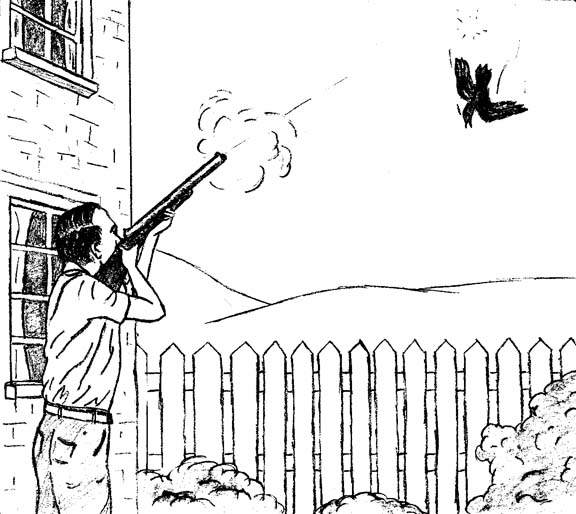
\includegraphics[width=0.95\columnwidth]{figures/exampleprompt2.jpg}\\
\hline
\textbf{Response (L1)} \\
\hline
The man killing the beard. (Arabic)\\
\hline
A man is shutting a bird. (Chinese) \\
\hline
A man is shooting a bird. (English) \\
\hline
The man shouted the bird. (Spanish)\\
\hline
\end{tabular}
\end{center}
\caption{Example item and responses}
\label{fig:example-picture}
\end{figure}

The PDT consists of 10 items (8 line drawings and 2 photographs\footnote{We have not observed substantial differences between responses for the drawings and the photographs.}) intended to elicit a single sentence
each; an example is given in Figure~\ref{fig:example-picture}. Participants
were asked to view the image and describe the action in past or present tense.
%, and care was
%taken to explain to participants that either past or present tense
%(and simple or progressive aspect) was acceptable. 
%Responses were typed by the participants themselves. 25 of the 39 NNS participants performed the task in a setting where automatic spell checking was disabled; the remaining 14 performed the task online on their own computers, and although they were instructed to disable spell checking, it is likely that a number of them did not.
%
% at Indiana University.
The data consist of responses from 53 informants (14 NSs, 39 NNSs),
for a total of 530 sentences, with the NNSs being intermediate and
upper-level adult English learners in an intensive English as a Second
Language program.  The distribution of first languages (L1s) is: 14
English, 16 Arabic, 7 Chinese, 2 Japanese, 4 Korean, 1 Kurdish, 1
Polish, 2 Portuguese, and 6 Spanish.
%\textbf{[(From 2013, verbatim. (END)]}

Responses were typed by the participants themselves, with spell checking disabled in some cases.  Even among the NNSs that used spell checking, a number of spelling errors resulted in real words. To address this, we use a spelling correction tool to obtain candidate spellings for each word, prune the candidates using word lists from the NS responses, recombine candidate spellings into candidate sentences, and evaluate these with a trigram language model (LM) to select the most likely intended response \citep{king:dickinson:14}.
%
%\subsection{Past Work}
%\citet{king:dickinson:13} and \citet{king:dickinson:14} did some work on this task.

\md{First crack at an annotation paragraph}
\lk{Honestly, I think it's perfect. We admit there's no inter-annotator info, but we don't go out of the way to draw attention to that...}

Once the responses had been collected, the NNS responses were
annotated for correctness, with respect to the content of the picture.
The lead author marked spelling and meaning errors which prevent a
complete mapping to correct information
\citep[see][]{king:dickinson:13}.  On the one hand, minor misspellings
are counted as incorrect (e.g., \textit{The artiest is drawing a
  \textbf{portret}}), while, on the other hand, the annotation does
not require distinguishing between between spelling and meaning
errors.  In the future, we plan on fine-tuning the annotation
criteria.
%, better accounting for strict meaning

\section{Generalizing the Methods}
\label{sec:ranking}

%The previous work assumed that the assessment of NNS responses
%involves determining whether the gold standard (GS) contains the same
%semantic triple that the NNS produced, i.e., whether a \textit{triple}
%is) \textit{covered} or \textit{non-covered}.  In such a situation the
%GS need only be comprised of \textit{types} of semantic triples.  As
%noted above, however, the GS is incomplete---meaning that exact
%matching is going to miss many cases, and indeed
%\citet{king:dickinson:13} note that GS coverage is only at 50.8\%.
%Additionally, relying on matching of triples limits the utility of the
%method to specific semantic requirements, namely transitive sentences.
%By moving to: i) bags of dependencies and: iii) tallying the counts of
%(NS) responses in the GS, we can move into: ii) a gradable, or
%ranking, approach to NNS responses.
The previous work assumed that the assessment of NNS responses
involves determining whether the gold standard (GS) contains the same
semantic triple that the NNS produced, i.e., whether a \textit{triple}
is \textit{covered} or \textit{non-covered}.  In such a situation the
GS need only be comprised of \textit{types} of semantic triples.  But
the GS is comprised of the small set of NS responses\md{I just noticed that I don't
  think we ever said that GS=NS responses}\lk{nice catch---that explains the reviewer's confusion} and is thus
incomplete---meaning that exact matching is going to miss many cases,
and indeed in \citet{king:dickinson:13}, we note
%\lk{Is this appropriate? I'm trying to de-anonymize a bit} 
% MD: Looks good!
that GS coverage is only at 50.8\%.  Additionally, relying on matching
of triples limits the utility of the method to specific semantic
requirements, namely transitive sentences.  By moving to bags of
dependencies and tallying the counts of (NS) responses in the GS, we
can move into a gradable, or ranking, approach to NNS responses.

We want to emphasize the degree to which a response conveys the same
meaning as the GS, necessitating an approach which can automatically
determine the importance of a piece of information in the GS.  We
break this down into how we represent the information
(section~\ref{sec:representation}) and then how we compare NNS
information to GS information (section~\ref{sec:scoring}), allowing us
to rank responses from least to most similar to the GS.\footnote{Although rankings often go from highest to lowest, we prioritize identifying problematic cases, so we rank accordingly.}  We also
discuss the handling of various other system parameters (section~\ref{sec:parameters}).

\subsection{Representation}
\label{sec:representation}

To overcome the limitations of an incomplete GS, we represent each
response as a list of \textit{terms} taken from the dependency parse
\citep{demarneffe:ea:06}, the terms referring to
%being either 
individual dependencies (i.e., relations between words).
%or individual words. 
This eliminates the complications of extracting semantic triples from
dependency parses, which could only handle a very restricted set of
grammatical forms and resulted in errors in 7--8\% of cases
\citep{king:dickinson:13}. Operating directly on individual
%words or
dependencies from the overall tree also means the system can allow for
``partial credit''; it distributes the matching over smaller,
overlapping pieces of information rather than a single, highly
specific triple.

Specifically, representations take one of five forms.  We first
tokenize and lemmatize the response to a list of lemmas that
represents the response.
%; we call this representation the \textbf{lemma} setting. 
The five term representations are then variations on dependencies. The
full form concatenates the label, head and dependent, as in
\texttt{subj\#boy\#kick}. We call this \textbf{ldh} (label, dependent,
head). The remaining four forms abstract over either the label, head
and/or dependent, as in \texttt{X\#boy\#kick}. We refer to these forms
as \textbf{xdh}, \textbf{lxh}, \textbf{ldx}, and \textbf{xdx}. 
%
The \param{xdx} model is on a par with treating the sentence as a bag
of lemmas, except that some function words not receiving parses (e.g.,
prepositions) are not included \citep[see][]{king:dickinson:13}.
%
In our current experiments, we test each of these term representations
separately, but we expect to ultimately make use of some weighted
combination. Future representations may also incorporate WordNet
relations or semantic role labeler output.

% Specifically, representations take one of five forms. In the simplest
% case, we tokenize and lemmatize the response to a list of lemmas that
% represents the response; we call this representation the
% \textbf{lemma} setting. The remaining four term representations are
% variations on dependencies. The full form concatenates the label, head
% and dependent, as in \texttt{subj\#boy\#kick}. We call this
% \textbf{ldh} (label, dependent, head). The remaining three forms
% abstract over either the label, head or dependent, as in
% \texttt{X\#boy\#kick}. We refer to these
% forms as \textbf{xdh}, \textbf{lxh} and \textbf{ldx}. In our current
% experiments, we test each of these term representations separately,
% but we expect to ultimately make use of some weighted
% combination. Future representations may also incorporate WordNet
% relations or semantic role labeler output.

\subsection{Scoring Responses}
\label{sec:scoring}

Taking the term representations from the previous section, the next
task is to combine them in a way which ranks responses from least to
most appropriate.  Responses are scored with one of four approaches,
using one of two methods to \textbf{weight} response terms combined
with one of two methods to \textbf{compare} the weighted NNS terms
with the GS.

% For weighting, we use either a simple frequency measure (\textbf{F})
% or a score based on what we term \textbf{importance} (\textbf{I}). The
% importance score is a simple measure in the vein of tf-idf, and we

For weighting, we use either a simple frequency measure (\textbf{F})
or one based on \textbf{tf-idf} (\textbf{T})
\citep[][ch. 6]{manning-et-al:08}.  We explore tf-idf as a measure of
a term's importance with the hope that it is able to reduce the impact
of semantically unimportant terms---e.g., determiners like
\textit{the}, frequent in the GS, but unimportant for evaluating the
semantic contents of NNS responses---and to upweight terms which may
be salient but infrequent, e.g., only used in a handful of GS
sentences. For example, for an item depicting a man shooting a bird
(see Table~\ref{tab:i10responses-avgprec} and Figure~\ref{fig:example-picture}), of 14 GS responses, 12
described the subject as \textit{man}, one as \textit{he} and one as
\textit{hunter}. Since \textit{hunter} is infrequent in English, even
one instance in the GS should get upweighted via tf-idf, and indeed it
does.
% \md{Double-check whether \textit{hunter} gets upweighted with tf-idf.}
% \lk{If this means ``is it ranked higher via tf-idf than via
%   frequency?'', then yes, and I reworded to reflect this.}
%allows us to upweight the term via a measure of importance. 
%Common words like \textit{he}, however, get downweighted. 
This is valuable, as numerous NNS responses use \textit{hunter}.

Calculating tf-idf relies on both \emph{term frequency} ($tf$) and
\emph{inverse document frequency} ($idf$).  Term frequency is simply
the raw count of an item, and for tf-idf of terms in the GS, we take
this as the frequency within the GS.  Inverse document frequency is
derived from some reference corpus, and it is based on the notion that
appearing in more documents makes a term less informative with respect
to distinguishing between documents.  The formula is in
(\ref{ex:tfidf}) for a term $t$, where $N$ is the number of documents
in the reference corpus, and $df_{t}$ is the number of documents
featuring the term ($idf_{t} = \log \frac{N}{df_{t}}$).  A term
appearing in fewer documents will thus obtain a higher $idf$ weight,
and this should readjust frequencies based on semantic importance.

\begin{exe}
  \ex\label{ex:tfidf} $tfidf(t) = tf_{GS} \log \frac{N}{df_{t}}$
  %, where $df_t = |\{d\in D, t \in d\}|$
\end{exe}

% To calculate the importance of a term in the GS, we first obtain a
% \textit{relative}
% % (or \textit{augmented}) 
% term frequency ($rtf$) in the GS by dividing the total number of the
% term's tokens in the GS by the total number of all tokens in the GS.
% We then incorporate the corpus frequency, adding relative term
% frequencies at the document level for each document ($d$) in the
% reference corpus ($Ref$), as shown in the numerator of
% (\ref{ex:importance}).
% % , and the sum of these
% % corpus document $rtf$ scores is added to the GS $rtf$ score
% Finally, this score is divided by the term's raw frequency in the
% entire corpus ($tf_{raw}$) to obtain the importance score.  This last
% step of division is essentially an inverse corpus frequency, and it is
% the factor which we hope readjusts frequencies based on semantic
% importance.
% \begin{exe}
%   \ex\label{ex:importance} $importance(term) = \frac{rtf_{GS} +
%     \sum\limits_{d \in Ref} rtf_d}{tf_{raw}}$
% \end{exe}

After counting/weighting, the frequencies are then either
\textbf{averaged} to yield a response score (\textbf{A}), or NNS term
weights and GS term weights are treated as vectors and the response
score is the \textbf{cosine distance} (\textbf{C}) between them.  This
yields:

%%former approach names: b = FA; m = IC (TC); c = FC; a = IA (TA)
\paragraph{Frequency Average (FA).} 
%This approach serves as our baseline. 
Within the GS, the frequency of each term is calculated. Each term in
the NNS response is then given a score equal to its frequency in the
GS; terms missing from the GS are scored zero. The response score is
the average of the term scores, with higher scores closer to the GS.

\paragraph{Tf-idf Average (TA).} This involves the exact same
averaging as with model FA, but now the terms in the GS are assigned
tf-idf weights before averaging.

\paragraph{Frequency Cosine (FC).} The frequency of each term is
calculated within the GS and (separately) within the NNS response. 
%\marginpar{\scriptsize{LK: above: "cosine distance (C)", so I changed "Comparison" (FC) to "Cosine". Good? I need to scan for other instances.}}
The term scores are then treated as vectors, and the response score is
the cosine distance between them, with lower scores being closer to
the GS.

\paragraph{Tf-idf Cosine (TC).} This involves the exact same
distance comparison as with model FC, but now the terms of both the GS
and NNS responses are assigned tf-idf weights before comparison.

\subsection{System Parameters}
\label{sec:parameters}

In addition to the four approaches, we have term representations and
two sets of parameters, listed below, to vary, resulting in a total of
60 settings for processing responses (see also
Table~\ref{tab:dist-ranked-parameters}). 
%\lk{As of 4/4, we now have 60 settings, not 52; i replaced a couple "52"s; watch out for other mentions}

\paragraph{Term form.} As discussed in
section~\ref{sec:representation}, the terms can take one of five
representations: \param{ldh}, \param{xdh}, \param{lxh}, \param{ldx},
or \param{xdx}.
%\param{lemma}, \param{ldh}, \param{xdh}, \param{lxh}, \param{ldx}.

\paragraph{Scoring approach.} As discussed in
section~\ref{sec:scoring}, the NNS responses can be
compared with the GS via models \param{FA}, \param{TA}, \param{FC}, or \param{TC}.

\paragraph{Reference corpus.} The reference corpus for deriving tf-idf
scores can be either the Brown Corpus \citep{kucera:francis:67} or the
Wall Street Journal (WSJ) Corpus \citep{marcus-et-al:93}. These are
abbreviated as \param{B} and \param{W} in the results
below; \param{na} indicates the lack of a reference corpus, as this is
only relevant to approaches \param{TA} and
\param{TC}. The corpora are divided into as many documents as
originally distributed (\param{W}: 1640, \param{B}: 499). The WSJ is
larger, but Brown has the benefit of containing more balance in its
genres (vs. newstext only). Considering the narrative nature of PDT
responses, a reference corpus of narrative texts would be ideal, but
we choose manually parsed reference corpora as they are more reliable
than automatically parsed data.

% \md{I'm pretty sure we're half non-anonymous at this point, and I
%   think we need to make clear there are details we're not going over
%   (for good reasons)}
% Update: I now see the spelling

\paragraph{NNS source.} Each response has an original version
(\param{NNSO}) and the output of a language model spelling corrector
%\texttt{+} module
(\param{NNSLM}) (see section~\ref{sec:data}).
% \citep{king:dickinson:14}. => cited in earlier section
 %%%for now, let's hide this for anonymity's sake?

\subsection{Results}

\subsubsection{Evaluation metrics}
\label{sec:metrics}

We ran 60 response experiments, each with different system settings
(section~\ref{sec:parameters}). Within each experiment, we rank the 39
scored NNS responses from least to most similar to the GS.
%\md{Do we want to add something parenthetical like ``least coming first to model error detection''? (I can't think how to say it concisely.)} 
\md{Could/Should the footnote go into section 3?}
\lk{It could, but I kinda like it here}
For assessing these settings themselves, we rely on past annotation,
which counted unacceptable responses as errors (see
section~\ref{sec:data}).\footnote{The source of the error is also
  labeled---stemming from NNS unintelligibility or a system error
  (from spelling correction, parsing, or some downstream
  component)---but we do not currently use this annotation.}  As the
lowest rank indicates the greatest distance from the GS, a good system
setting should ideally position the unacceptable responses among those
with the lowest rankings. Thus, we assign each error-containing
response a score equal to its rank, or, if necessary, the average rank
of responses sharing the same score.

In Table~\ref{tab:i10responses-avgprec}, an excerpt of sentence
responses is shown for one item, ranked from lowest to highest.  To
take one example, the third-ranked sentence, \textit{the man is hurting duck}, has a score of 0.996, and it is annotated as an error (1 in
the \textit{E} column).  Thus, the evaluation metric adds a score of 3
to the overall sum.  The sentence ranked 18, by contrast, is not an
error, and so nothing is added.  In the case of the top rank, two
responses with errors are tied, covering rank 1 and 2, so each adds a score of 1.5.

\begin{table}[htb!]
\begin{center}
\setlength{\tabcolsep}{0.3em}
\begin{tabular}{|r|c|l|r|r|}
 \hline
 \textit{R} & \textit{S} & Sentence & \textit{E} & \textit{V}\\
 \hline
 \hline
\multirow{2}{*}{1} & 1.000 & she is hurting. & 1 & 1.5 \\
& 1.000 & man mull bird & 1 & 1.5 \\
\hline
3 & 0.996 & the man is hurting duck. & 1 & 3.0 \\
4 & 0.990 & he is hurting the bird. & 1 & 3.0 \\
\hline
11 & 0.865 & the man is trying to hurt a bird & 1 & 11.0 \\
12 & 0.856 & a man hunted a bird. & 0 & 0.0 \\
\hline
17 & 0.775 & the bird not shot dead.  & 1 & 17.0 \\
18 & 0.706 & he shot at the bird & 0 & 0.0 \\
19 & 0.669 & a bird is shot by a un & 1 & 19.0 \\
20 & 0.646 & the old man shooting the birds & 0 & 0.0 \\
\hline
37 & 0.086 & the old man shot a bird. & 0 & 0.0 \\
38 & 0.084 & a old man shot a bird. & 0 & 0.0 \\
39 & 0.058 & a man shot a bird & 0 & 0.0 \\
  \hline
  \hline
  \multicolumn{3}{|c|}{Total (Raw)} & 17 & 169 \\
  \hline
  \multicolumn{3}{|c|}{Average Precision} & \multicolumn{2}{c|}{0.75084} \\
 \hline
\end{tabular}
\caption{Rankings for Item 10 from the best system setting (TC\_B\_NNSLM\_ldh) based on average precision scores. \textit{R}: rank; \textit{S}: sentence score; \textit{E}: error; \textit{V}: rank value. }
%%LK: fixed 4/6 pm.
\label{tab:i10responses-avgprec}
\end{center}
\end{table}

The sum of these scores is taken as the \textbf{Raw} metric for that
experimental setting. In many cases, one version of a response
(\param{NNSO} or \param{NNSLM}) contains an error, but the other
version does not. Thus, for example, an \param{NNSO} experiment may
result in a higher error count than the \param{NNSLM} equivalent, and
in turn a higher Raw score.
% for the settings. 
In this sense, Raw scores emphasize error reduction and incorporate
item difficulty.
%  for settings

However, it is possible that the \param{NNSO} experiment, even with
its higher error count and Raw score, does a better job ranking the
responses in a way that separates good and erroneous ones. To account
for this, we also use \textbf{(mean) average precision ((M)AP)}
\citep[][ch. 8]{manning-et-al:08}, which emphasizes discriminatory
power.
% rather than error reduction.

For average precision (AP), one calculates the precision of error
detection at every point in the ranking, lowest to highest.  In
Table~\ref{tab:i10responses-avgprec}, for example, the precision for
the first cut-off (1.000) is 1.0, as two responses have been
identified, and both are errors ($\frac{2}{2}$). At the 11th- and
12-ranked response, precision is 1.0 ($\frac{11}{11}$) and 0.917
(=$\frac{11}{12}$), respectively, precision dropping when the item is
not an error.
% For the next cutoff, the precision is 0.75, as three out of four
% identified items are errors.  
AP averages over the precisions for all $m$ responses ($m=39$ for our
NNS data), as shown in (\ref{ex:ap}), with each response notated as
$R_k$.  Averaging over all 10 items results in the Mean AP (MAP).

\begin{exe}
  \ex\label{ex:ap} $AP(item) = \frac{1}{m} \sum\limits_{k=1}^m
  Precision(R_k)$
\end{exe}

% devise a \textbf{Normalized} metric that emphasizes this
% discriminatory power rather than error reduction.  Normalized scoring
% relies on comparing the Raw scores to best and worst case scenarios.

% Specifically for this metric, we first count the number of erroneous
% responses ($n$) the settings must handle; for the item in
% table~\ref{tab:i10responses-avgprec}, for example, $n=17$. The best
% possible ranking ($R_b$) for errors is $1$ through $n$ (e.g., the
% lowest 17 cases), and the worst possible ranking ($R_w$) is at the
% bottom of the scale, $39-n$ through $39$.
% % (e.g., ranks 23--39).  
% We sum the best and worst rank lists and take their difference; for
% $n=17$, for example, the best model sum is $153$
% ($= \sum_{i=1}^{17} i$) and the worst is $527$
% ($= \sum_{i=23}^{39} i$), giving a difference of $374$, notated as
% $D_w$.  We obtain the difference for the actual ranking, $R_a$, in the
% same way, giving $D_a$.  In this case, for example,
% $D_a = 163 - 153 = 10$.  This indicates how far off the actual ranking
% $R_a$ is from the best one.  To obtain a score between $0$ and $1$, we
% finally divide by $D_w$ to arrive at a final Normalized score.  In
% this case, we obtain $\frac{10}{527} = 0.02674$.

As mentioned, the Raw metric emphasizes error reduction, as it
reflects not just performance on identifying errors, but also the
effect of the overall number of errors.  In this way, it may be useful
for predicting future system performance, an issue we explore in the
evaluation of clustering items (section~\ref{sec:clusteringresults}).
MAP, on the other hand, emphasizes finding the optimal separation
between errors and non-errors and is thus more of the focus in the
evaluation of the best system parameters next.
%, discussed next.

\subsubsection{Best system parameters} 
%Results}

To start the search for the best system parameters, it may help to
continue our single example, in
Table~\ref{tab:i10responses-avgprec}. The best setting, as determined by the
Normalized metric, uses the tf-idf cosine (\param{TC}) approach with the Brown Corpus (\param{B}),
the spelling corrected response (\param{NNSLM}), and the full form of
the dependencies (\param{ldh}). It ranks highest because errors are
well separated from non-errors; the highest ranked of 17 total errors
is at rank 19.  Digging a bit deeper, we can see in this example how
the verb \textit{shoot} is common in all the highest-ranked cases shown
(\#37--39), but absent from all the lowest, showing both the effect of
the GS (as all NSs used \textit{shoot} to describe the action) and the
potential importance of even simple representations like lemmas.  In
this case, the \param{ldh} representation is best, likely because the
word \textit{shoot} is not only important by itself, but also in terms
of which words it relates to, and how it relates (e.g.,
\texttt{dobj\#bird\#shoot}).

\begin{table*}
\begin{center}
\begin{tabular}{|l|r||l|r||l|r||l|r|}
 \hline
 \multicolumn{2}{|c||}{Approach} & \multicolumn{2}{|c||}{Term Form} & \multicolumn{2}{|c||}{Ref. Corpus (TA/TC)} & \multicolumn{2}{|c|}{NNS Source} \\
 \hline
 \hline
 0.51577 & TC & xdh & 0.51810 & Brown & 0.51534 & NNSLM & 0.51937 \\
 \hline
 0.50780 & FC & ldh & 0.51677 & WSJ & 0.50798 & NNSO & 0.49699 \\
 \hline
 0.50755 & TA & lxh & 0.51350 & & & & \\
 \hline
 0.49464 & FA & xdx & 0.49901 & & & & \\
 \hline
 & 	& ldx & 0.49352 &  &  &  & \\
 \hline
\end{tabular}
\caption{Approaches and parameters ranked by mean average precision for all 10 PDT items.}
%%LK: fixed 4/6 pm
\label{tab:dist-ranked-parameters}
\end{center}
\end{table*}

Table~\ref{tab:all-dist-ranked-settings} shows the five best and five
worst system settings averaged across all 10 PDT items, as ranked by
MAP. Among the trends that pop out is a favoritism
towards \param{NNSLM} models (i.e., spelling correction). This is due
to the fact that higher numbers of errors inflate the MAP scores, and
somewhat counterintuitively, the spelling correction module introduces
more errors than it corrects, meaning there are more errors present
overall in the \param{NNSLM} responses than in the \param{NNSO}
responses.\footnote{Note that among the remaining parameter classes,
  variation does not effect the number of errors.}

% \lk{not exactly sure what to say here, but I feel that this should be
%   pointed out somehow...}  \md{This may tie in to my comment later on
%   different ranges ...}
%A few general trends pop out, namely: a
%favoritism towards \param{NNSLM} models (i.e., spelling
%correction)---likely due to better downstream parsing based on correct
%spellings---
%%and the \param{xdh} dependency representation.  This
%representation means that the head and dependent words are linked, but
%the specific label is less important---likely covering variation in
%the syntactic tree (e.g., \texttt{nsubj} vs. \texttt{nsubjpass}
%[passive subject] for the same pair of words).  
Another feature among the best settings is the inclusion of heads in the dependency representations. In fact, the top 17 ranked settings all include heads (\param{lxh}, \param{xdh}, \param{ldh}); \param{xdx} first enters the rankings at 18, and \param{xdx} and \param{ldx} are common among the worst performers. This is likely due to the salience of the verbs in these transitive sentences; they constitute the heads of the subjects and objects, in relatively short sentences with few dependencies.
Furthermore, the tf-idf weighted models dominate the rankings, especially \param{TC}. It is also clear that for our data tf-idf works best with the Brown Corpus (\param{B}).
%Furthermore, our importance weights seem less helpful here, with \param{FA}
%and \param{FC} models at the top and \param{IA} and \param{IC} at the
%bottom.

%\begin{table}[htb!]
%\begin{center}
%\begin{tabular}{|r|r|c|}
% \hline
% Rank & Score & Settings \\
% \hline
% \hline
% 1 & 0.120794037 & FC\_na\_NNSLM\_xdh \\
% \hline
% 2 & 0.122105776 & FA\_na\_NNSLM\_xdh \\
% \hline
% 3 & 0.125286986 & FA\_na\_NNSLM\_ldh \\
% \hline
% 4 & 0.126513148 & FC\_na\_NNSLM\_lxh \\
% \hline
% 5 & 0.126863051 & FA\_na\_NNSLM\_lxh \\
% \hline
%% 6 & 0.127294301 & FC\_na\_NNSLM\_ldh \\
%% \hline
%% 7 & 0.149902623 & FA\_na\_NNSLM\_lemma \\
%% \hline
%% 8 & 0.154534502 & FC\_na\_NNSO\_ldh \\
%% \hline
%% 9 & 0.154835099 & FA\_na\_NNSO\_ldh \\
%% \hline
%% 10 & 0.157323338 & FA\_na\_NNSO\_xdh \\
% \hline
% 48 & 0.218474550 & IC\_W\_NNSO\_ldx \\
% \hline
% \multirow{2}{*}{49} & 0.222587120 & IA\_W\_NNSO\_lxh \\
% \cline{2-3}
% & 0.222587120 & IC\_W\_NNSO\_lxh \\
% \hline
% \multirow{2}{*}{51} & 0.233852894 & IA\_W\_NNSLM\_ldx \\
% \cline{2-3}
%  & 0.233852894 & IC\_W\_NNSLM\_ldx \\
% \hline
%\end{tabular}
%\caption{Based on the Normalized metric, the five best and five worst settings, averaged across all 10 PDT items.}
%\label{tab:all-dist-ranked-settings}
%\end{center}
%\end{table}
%
\begin{table}[htb!]
\begin{center}
\begin{tabular}{|r|l|c|}
 \hline
 Rank & MAP & Settings \\
 \hline
 \hline
1 & 0.5534 & TC\_B\_NNSLM\_lxh \\
\hline
2 & 0.5445 & TA\_B\_NNSLM\_lxh \\
\hline
3 & 0.5435 & TC\_W\_NNSLM\_lxh \\
\hline
4 & 0.5422 & TC\_B\_NNSLM\_xdh \\
\hline
5 & 0.5368 & TC\_B\_NNSLM\_ldh \\
 \hline
 \hline
56 & 0.4816 & TA\_B\_NNSO\_xdx \\
\hline
57 & 0.4796 & FA\_na\_NNSLM\_ldx \\
\hline
58 & 0.4769 & FC\_na\_NNSO\_lxh \\
\hline
59 & 0.4721 & TA\_W\_NNSO\_xdx \\
\hline
60 & 0.4530 & FA\_na\_NNSO\_lxh \\
\hline
\end{tabular}
\caption{Based on Mean Average Precision, the five best and five worst settings across all 10 PDT items.}
%%LK: fixed 4/6 pm
\label{tab:all-dist-ranked-settings}
\end{center}
\end{table}

We also summarize the rankings for the individual parameter classes,
presented in Table~\ref{tab:dist-ranked-parameters}, confirming the
trends in Table~\ref{tab:all-dist-ranked-settings}. For a given
parameter, e.g., \param{ldh}, we averaged the experiment scores from
all settings including \param{ldh} across all 10 items. Notably, \param{TC} outperforms the other models, with \param{FC} and \param{TA} close behind (and nearly tied). Performance falls for the simplest model, \param{FA}, which was in fact intended as a baseline. With \param{TC}$>$\param{FC} and \param{TA}$>$\param{FA}, tf-idf weighting seems preferable to basic frequencies.

Again, the importance of including heads in dependencies is apparent here; the three dependency representations containing heads constitute the top three, with a sizable drop in performance for the remaining two forms (\param{xdx} and \param{ldx}). Moreover, given the content and narrative style of the PDT responses, it is unsurprising that the Brown Corpus serves as a better reference corpus than the WSJ Corpus for tf-idf. Finally, the \param{NNSLM} source significantly outperforms the \param{NNSO} source.
%Notably, \param{FA} and \param{FC} appear to be the strongest
%approaches, and the difference between these two is closer than the
%difference between either \param{F} approach and either \param{I}
%approach. This suggests that our implementation of the term importance
%metric should be reconsidered in the future (e.g., tf-idf or a similar
%measure might offer some improvement here). We also observe that the
%\param{xdh} and \param{ldh} terms outperform other forms, indicating
%that matching an NNS response dependent-head relationship to the GS is
%a strong measure of the quality of the response.

% \marginpar{MD: If we run out of space,
%   Table~\ref{tab:raw-ranked-parameters} and discussion can be cut.}

% It is instructive to examine the rankings by the Raw metric, as we see
% a slightly different picture for ...

% \begin{itemize}
% \item the Raw metric gives a slightly different picture ...
% \item methods of evaluating the ranking---non-normalized
%   vs. normalized---mostly show the same trends, except that the
%   best representation (lemmas vs. xdh) changes
% \end{itemize}

% \begin{table*}
% \begin{center}
% \begin{tabular}{|l|r||l|r||l|r||l|r|}
%  \hline
%  \multicolumn{2}{|c||}{Approach} & \multicolumn{2}{|c||}{Term Form} & \multicolumn{2}{|c||}{IA/IC Ref.} & \multicolumn{2}{|c|}{NNS Source} \\
%  \hline
%  \hline
%  FA & 160.38 & lemma & 165.80 & Brown & 173.24 & LM & 165.96 \\
%  \hline
%  FC & 163.84 & xdh & 165.83 & WSJ & 176.25 & Orig & 173.81 \\
%  \hline
%  TA & 174.74 & ldh & 166.17 & & & & \\
%  \hline
%  TC & 174.74 & lxh & 169.89 & & & & \\
%  \hline
%  & 	& ldx & 179.02 & & & & \\
%  \hline
% \end{tabular}
% \caption{Approaches and parameters ranked by the Raw metric, averaged across all 10 PDT items.}
% \label{tab:raw-ranked-parameters}
% \end{center}
% \end{table*}

Despite the strength of these overall trends, variability
does exist among the best settings for different items, a point obscured
in the averages.  In Tables~\ref{tab:i01-dist-ranked-settings} and
\ref{tab:i05-dist-ranked-settings}, we present the best and worst
ranked settings for two of the least similar items, 1 and 5.
% Both share a preference for the spelling-corrected \param{NNSLM}
% responses.
Their dissimilarity can be seen at a glance, simply from the range of
the AP scores (0.05--0.31 for item 1 vs. 0.52--0.81 for item 5), which
in itself reflects a differing number of erroneous responses (2 [\param{NNSO}]
or 6 [\param{NNSLM}] for item 1 vs. 23 or 24 for item 5).

%\md{Do we have a story for why the ranges are so different?}

For item 1, a drawing of a boy kicking a ball, we see considerable
variability in the best approach just within the top five settings:
all four approaches are in the top five.  Contrary to the overall
trends, we also see the \param{ldx} form---without any head
information---in the two best settings.  Note also that, even though
tf-idf weighting (\param{TA}/\param{TC}) is among the best settings, it is
consistently the worst setting, too.

%... \lk{I'm stuck here... considering changing one of these to better illustrate variation}
%the top five settings all use
%the \param{FA} approach; \param{FC} settings are also quite strong
%(but absent from the table). \param{NNSO} settings tie for the top
%three positions, with variation in \param{ldh}, \param{lxh}
%and \param{xdh} making no difference. Lemmas are absent from the top
%five (they first appear at rank 14), and \param{ldx} measures are
%similarly weak (as in most cases).

% \begin{itemize}
% \item Although NNSLM$>$NNSO in both
% \item \param{xdx} for item 5
% \item tf-idf the worst five for item 1 (also among the best, though)
% %\item much different overall precisions!
% \end{itemize}

For item 5 in Table~\ref{tab:i05-dist-ranked-settings}, a drawing of a
man raking leaves, the most noticeable difference is that
of \param{xdx} being among three of the top five settings.
% \param{NNSLM} is the best predictor of a strong setting performance,
% and the first \param{NNSO} setting appears at rank 15. The approach is
% highly variable, with all four approaches
% (\param{FA}, \param{FC}, \param{IA}, \param{IC}) appearing in the top
% five. \param{Lemma}s perform unusually well here, as do \param{lxh}
% terms, and among the \param{I} approaches, the \param{B}rown Corpus
% outperforms the \param{W}SJ Corpus (as usual).
We believe that part of the reason for
% the differing performance, e.g., 
the superior performance of \param{xdx} (cf. lemmas), is that for this
item, all the NSs use the verb \textit{rake}, while none of the NNSs use this word.  For item 1 (the boy kicking a ball), there is lexical variation
for both NSs and NNSs.
%
%\begin{table}[htb!]
%\begin{center}
%\begin{tabular}{|r|r|c|}
% \hline
% Rank & Score & Settings \\
% \hline
% \hline
% \multirow{3}{*}{1} & 0.067567568 & FA\_na\_NNSO\_ldh \\
% \cline{2-3}
% & 0.067567568 & FA\_na\_NNSO\_lxh \\
% \cline{2-3}
% & 0.067567568 & FA\_na\_NNSO\_xdh \\
% \hline
% 4 & 0.070707071 & FA\_na\_NNSLM\_lxh \\
% \hline
% 5 & 0.075757576 & FA\_na\_NNSLM\_ldh \\
% \hline
% \hline	
% \multirow{3}{*}{47} & 0.189189189 & IA\_W\_NNSO\_ldx \\
% \cline{2-3}
% & 0.189189189 & IC\_W\_NNSO\_ldh \\
% \cline{2-3}
% & 0.189189189 & IC\_W\_NNSO\_ldx \\
% \hline
% \multirow{2}{*}{51} & 0.22972973 & IA\_W\_NNSO\_xdh \\
% \cline{2-3}
%  & 0.22972973 & IC\_W\_NNSO\_xdh \\
% \hline
%\end{tabular}
%\caption{Based on the Normalized metric, the five best and five worst settings for item 1.}
%\label{tab:i01-dist-ranked-settings}
%\end{center}
%\end{table}

\begin{table}[htb!]
\begin{center}
\begin{tabular}{|r|c|c|}
 \hline
 Rank & AP & Settings \\
 \hline
 \hline
% \multirow{3}{*}{1} & 0.067567568 & FA\_na\_NNSO\_ldh \\
% \cline{2-3}
% & 0.067567568 & FA\_na\_NNSO\_lxh \\
1 & 0.30997 & TC\_B\_NNSLM\_ldx \\
\hline
2 & 0.30466 & TA\_B\_NNSLM\_ldx \\
\hline
3 & 0.30015 & TA\_B\_NNSLM\_xdh \\
\hline
4 & 0.29704 & FC\_na\_NNSLM\_xdh \\
\hline
5 & 0.29650 & FA\_na\_NNSLM\_ldh \\
 \hline
 \hline
56 & 0.06474 & TC\_B\_NNSO\_ldx \\
\hline
57 & 0.06174 & TC\_W\_NNSO\_ldx \\
\hline
58 & 0.06102 & TA\_W\_NNSO\_lxh \\
\hline
59 & 0.05603 & TA\_W\_NNSO\_xdx \\
\hline
60 & 0.05094 & TA\_W\_NNSO\_ldx \\
 \hline
\end{tabular}
\caption{Based on Average Precision, the five best and five worst settings for item 1.}
%%LK: fixed 4/6 pm
\label{tab:i01-dist-ranked-settings}
\end{center}
\end{table}

%\begin{table}[htb!]
%\begin{center}
%\begin{tabular}{|r|r|c|}
% \hline
% Rank & Score & Settings \\
% \hline
% \hline
% 1 & 0.147222222 & FA\_na\_NNSLM\_lemma \\
% \hline
% 2 & 0.158333333 & FA\_na\_NNSLM\_lxh \\
% \hline
% 3 & 0.181944444 & FC\_na\_NNSLM\_lxh \\
% \hline
% \multirow{2}{*}{4} & 0.197222222 & IA\_B\_NNSLM\_lxh \\
% \cline{2-3}
% & 0.197222222 & IC\_B\_NNSLM\_lxh \\
% \hline
% \hline
% 47 & 0.448369565 & IC\_W\_NNSO\_lxh \\
% \hline
% 49 & 0.46875 & FC\_na\_NNSO\_lxh \\
% \hline
% 50 & 0.47826087 & FA\_na\_NNSO\_lxh \\
% \hline
% \multirow{2}{*}{51} & 0.486413043 & IA\_B\_NNSO\_lxh \\
% \cline{2-3}
% & 0.486413043 & IC\_B\_NNSO\_lxh \\
% \hline
%\end{tabular}
%\caption{Based on the Normalized metric, the five best and five worst settings for item 5.}
%\label{tab:i05-dist-ranked-settings}
%\end{center}
%\end{table}
\begin{table}[htb!]
\begin{center}
\begin{tabular}{|r|c|c|}
 \hline
 Rank & AP & Settings \\
 \hline
 \hline
 1 & 0.80965 & FA\_na\_NNSLM\_xdx \\
 \hline
 2 & 0.80720 & TA\_B\_NNSLM\_lxh \\
 \hline
 3 & 0.80473 & TC\_B\_NNSLM\_lxh \\
 \hline
 4 & 0.79438 & TC\_B\_NNSLM\_xdx \\
 \hline
 5 & 0.78108 & TC\_W\_NNSLM\_xdx \\
 \hline
 \hline 
 56 & 0.56495 & FC\_na\_NNSO\_xdh \\
 \hline
 57 & 0.56414 & TC\_B\_NNSO\_lxh \\
 \hline
 58 & 0.55890 & TC\_W\_NNSO\_lxh \\
 \hline
 59 & 0.54506 & FC\_na\_NNSO\_lxh \\
 \hline
 60 & 0.52013 & FA\_na\_NNSO\_lxh \\
 \hline
\end{tabular}
\caption{Based on Average Precision, the five best and five worst settings for item 5.}
%%LK: fixed 4/6 pm.
\label{tab:i05-dist-ranked-settings}
\end{center}
\end{table}

These types of differences---for these items and others---%
% ---indicative of what can be found comparing many different
% items---
lead us to explore the clustering of item patterns, in order to
leverage these differences and automatically choose the optimal
settings for new items; we turn to this next.
%in Section~\ref{sec:clusteringresults}.

\section{Clustering}
\label{sec:clustering}

Given the variability of NS and NNS responses, and the possible
correlation with different system parameters, we have begun exploring
connections by clustering the different items.  The clustering uses,
for one set, \emph{response features}, i.e., features observable from
the responses, and, separately, \emph{performance features}, i.e., the
performance of different system settings on the responses.
%
% conduct a number of hierarchical clustering experiments on the items
% in order 
%
Although the work is very exploratory, our goal is to get a handle on
learner variability for different items and explore correlations
between response and performance clusters.

%item clusters and best-performing system settings.

\subsection{Response Clustering}

We cluster the 10 PDT items using simple features taken from the
responses themselves. Specifically, we use various combinations of
type counts, token counts, and type-to-token ratios for each term form
(\param{ldh}, \param{xdh}, \param{lxh}, \param{ldx}, \param{xdx}),
taken from each response source (GS, \param{NNSO}, \param{NNSLM}).

\subsection{Performance Clustering}

From the system output, we cluster items using per-item Raw 
scores for various settings. That is, for each of the 10 items, we
calculate an average error score for each approach
(\param{FA}, \param{TA}, \param{FC}, \param{TC}), each term form
(\param{ldh}, \param{xdh}, \param{lxh}, \param{ldx}, \param{xdx}),
each reference corpus (\param{B}, \param{W}), and each
response source (\param{NNSO}, \param{NNSLM}). 
% \lk{Does this hold true now that we changed to MAP? I removed the footnote bc we haven't clustered by MAP...} These Raw scores
% parallel the rankings of the MAP scores presented in
% Table~\ref{tab:dist-ranked-parameters}, but, 
As mentioned in section~\ref{sec:metrics}, Raw scores should account for the number of
errors produced by NNSs for each item, which should 
correlate with future system performance.
%\footnote{Indeed, in initial experiments, clustering based on Normalized scores produced more noise than Raw ones.}

%\marginpar{MD: put this table here for now: I cut it later, but I see
%  it referenced here}

%\begin{table*}
%\begin{center}
%\begin{tabular}{|l|r||l|r||l|r||l|r|}
% \hline
% \multicolumn{2}{|c||}{Approach} & \multicolumn{2}{|c||}{Term Form} & \multicolumn{2}{|c||}{IA/IC Ref.} & \multicolumn{2}{|c|}{NNS Source} \\
% \hline
% \hline
% FA & 160.38 & lemma & 165.80 & Brown & 173.24 & LM & 165.96 \\
% \hline
% FC & 163.84 & xdh & 165.83 & WSJ & 176.25 & Orig & 173.81 \\
% \hline
% TA & 174.74 & ldh & 166.17 & & & & \\
% \hline
% TC & 174.74 & lxh & 169.89 & & & & \\
% \hline
% & 	& ldx & 179.02 & & & & \\
% \hline
%\end{tabular}
%\caption{Approaches and parameters ranked by the Raw metric, averaged across all 10 PDT items.}
%\label{tab:raw-ranked-parameters}
%\end{center}
%\end{table*}

\subsection{Results}
\label{sec:clusteringresults}
% \textbf{LK: MD, Could address the choice to use Raw scores for clustering? You have a better grasp at this point.}

Although there is noise in some experiments, some patterns do seem to
emerge in many of the clusterings; we present some of the most common
patterns here.
%
% Our primary reason for clustering PDT items is to find connections
% between features of the responses themselves and the performance of
% system settings on the responses. We tried this clustering using
% various combinations of features. Some seem to produce noise, but
% patterns did emerge in many of the clusterings; we present some of the
% most common patterns in the examples
% here.
Figure~\ref{fig:response-clusters} shows a clustering based on
response features that shares some characteristics with
Figure~\ref{fig:parameter-clusters}, a clustering based on performance
features. (Note that clustering heights are not to scale.)  In both
examples, items 5 and 9 form a cluster attaching to the root. These
are described in the GS as \textit{A man is raking leaves} and
\textit{Two boys are rowing a boat}. These were also the two most
difficult items for NNSs. While other items involved common verbs like
\textit{kick}, \textit{paint} and \textit{cut}, the actions depicted
in these items were more specific and required words outside the
vocabulary of many participants. For example, while all 14 NSs used
either \textit{row} or \textit{paddle}, only five of 39 NNSs used
these verbs; the rest used verbs like \textit{boat}, \textit{sail},
\textit{sit}, \textit{play} or \textit{ride}.

\begin{figure}
\begin{center}
\begin{tikzpicture}[sloped]
\node (5) at (-7.5,0) {5};
\node (9) at (-6.9,0) {9};
\node (1) at (-6.2,0) {1};
\node (4) at (-5.5,0) {4};
\node (6) at (-4.7,0) {6};
\node (2) at (-4.0,0) {2};
\node (8) at (-3.2,0) {8};
\node (10) at (-2.6,0) {10};
\node (3) at (-1.8,0) {3};
\node (7) at (-1.1,0) {7};
\node (59) at (-7.2,0.7) {};
\node (14) at (-5.9,0.7) {};
\node (28) at (-3.5,0.7) {};
\node (37) at (-1.5,0.7) {};
\node (1037) at (-2.3,1) {};
\node (281037) at (-2.9,1.3) {};
\node (6281037) at (-3.6,1.7) {};
\node (146281037) at (-4.9,2.1) {};
\node (59146281037) at (-6.4,2.5) {};
\draw  (5)  |- (59.center);
\draw  (9)  |- (59.center);
\draw  (1)  |- (14.center);
\draw  (4)  |- (14.center);
\draw  (2)  |- (28.center);
\draw  (8)  |- (28.center);
\draw  (3)  |- (37.center);
\draw  (7)  |- (37.center);
\draw (10) |- (1037.center);
\draw (37) |- (1037.center);
\draw (1037) |- (281037.center);
\draw (28) |- (281037.center);
\draw (6) |- (6281037.center);
\draw (281037) |- (6281037.center);
\draw (14) |- (146281037.center);
\draw (6281037) |- (146281037.center);
\draw (59) |- (59146281037.center);
\draw (146281037) |- (59146281037.center);
\end{tikzpicture}
\end{center}
\caption{PDT items clustered by type and token counts of all NS, NNSO and NNSLM responses.} 
%%duh?%%(Heights not to scale.)}
\label{fig:response-clusters}
\end{figure}

\begin{figure}
\begin{center}
\begin{tikzpicture}[sloped]
\node (5) at (-7.5,0) {5};
\node (9) at (-6.9,0) {9};
\node (3) at (-6.2,0) {8};
\node (8) at (-5.5,0) {3};
\node (2) at (-4.7,0) {2};
\node (10) at (-4.0,0) {10};
\node (1) at (-3.2,0) {1};
\node (4) at (-2.6,0) {4};
\node (6) at (-1.8,0) {6};
\node (7) at (-1.1,0) {7};
\node (59) at (-7.2,.8) {};
\node (210) at (-4.3,.7) {};
\node (14) at (-2.9,.7) {};
\node (67) at (-1.5,.7) {};
\node (8210) at (-4.9,1.0) {};
\node (38210) at (-5.7,1.3) {};
\node (1467) at (-2.2,1.4) {};
\node (382101467) at (-4,2) {};
\node (all) at (-5,2.5) {};
\draw  (5) |- (59.center);
\draw  (9) |- (59.center);
\draw  (2) |- (210.center);
\draw  (10) |- (210.center);
\draw  (1) |- (14.center);
\draw  (4) |- (14.center);
\draw  (6) |- (67.center);
\draw  (7) |- (67.center);
\draw  (8) |- (8210.center);
\draw  (210) |- (8210.center);
\draw  (8210) |- (38210.center);
\draw  (3) |- (38210.center);
\draw  (14) |- (1467.center);
\draw  (67) |- (1467.center);
\draw  (38210) |- (382101467.center);
\draw  (1467)  |- (382101467.center);
\draw  (59)  |- (all.center);
\draw  (382101467)  |- (all.center);
\end{tikzpicture}
\end{center}
\caption{PDT items clustered by parameter performance.} 
%%duh?%%(Heights not to scale.)}
\label{fig:parameter-clusters}
\end{figure}

Items 1 and 4 also appear as a cluster in both cases. In GS examples,
these are described as \textit{The boy is kicking a ball} and
\textit{A man is reading a newspaper}. The images portray actions that
language learners often learn in beginner courses, and in fact, these
were the easiest items for NNSs. The simple actions and objects mean
that both token counts and type counts are relatively low. \md{Just to make sure: are these still the right parameters that perform highly?}\lk{I changed it slightly; these are best, but the trend isn't very strong via MAP. the trends are different via Raw, (and stronger, hence the cluster!) but I don't think we want to go into that, given that we present the MAP for item 1 in Table 4} With regard
to feature performance, for both items the same parameters perform
highly (\param{TC}/\param{TA}, \param{ldx}/\param{ldh}/\param{xdh}), suggesting that a future item
which clusters with these two would benefit from the same processing.

%\subsection{Discussion}

\section{Summary and Outlook}

We have investigated ways to reason about learner meaning in cases
where the set of correct meanings is incomplete, namely in the
case of picture description tasks (PDTs).  Specifically, we have
explored different models of representing and scoring NNS responses to
a picture---different linguistic representations, term weighting
schemes, reference corpora, and use of spelling correction---in order
to automatically determine the relevant parts of an image from a set
of NS responses.  In more exploratory work, we have also examined the
variability in both NS and NNS responses, and how different system
parameters correlate with the variability.  

Already, the results are providing insight for future system
development, data collection, and investigations into learner
language.  A big next step of the work is to collect more data, and
examining the variability in the NS/NNS data has provided feedback on
the types of new data to gather, to better ensure a wide range of
behavior from NNSs.  Getting a range of items, with different sentence
types and variability in responses, will help us properly find our
envisioned sweet spot of semantic analysis.  In that vein, we plan on
exploring more parameters (e.g., semantic role information) and
holding out data to better gauge the impact of clustering a new item
with the existing items and selecting the processing parameters on
that basis.
%
Beyond that loom large questions about how to annotate gradability in
learner responses and how to map system processing to accurate
semantic feedback.

%We are still far from finding a 

% In this paper, we start on a path towards finding a ``sweet spot'' of
% semantic analysis \citep[cf.][]{bailey:meurers:08} for such
% image-based learner productions.
% % (CITE captioning-esque work?).
% In particular, using available NLP tools.
% %to build a shallow semantic analysis,
% %(for interactive sentences) 
% we move away from specific correct semantic representations and an
% exact definition of correctness, to more abstract data representations
% and more gradable notions of correctness (section~\ref{sec:ranking}).
% A benefit of more abstract representations is that they allow correct
% and relevant information to be derived from a relatively small set of
% native speaker responses, as opposed to deriving them by hand, in
% addition to allowing for a range of sentence constructions.

% a few more parameters (e.g., tf-idf)

% new data collection!

% We expect that further experiments with clustering items (and perhaps parameters) will reveal more patterns in the data. Ultimately, we expect to place unannotated responses from new items into known clusters, which would allow us to predict the optimal system settings, and possibly even the optimal threshold for acceptable responses.

% \begin{itemize}
% \item Future: leave-one-out testing: cluster unseen item with one of
%   other nine and use the best model of its closest match: see what
%   that performance is ...
% \end{itemize}

\section*{Acknowledgments}

We would like to thank the members of the CLingDing discussion group and the three anonymous reviewers for their helpful feedback.

{\fontsize{10}{1em}
\selectfont
\bibliography{levi-bib}
\bibliographystyle{styles/aclnatbib}
}

%\section*{Leftovers}

\end{document}
